\section{Introduction}
\begin{frame}{}
    \LARGE Image Segmentation: \textbf{Introduction}
\end{frame}

\begin{frame}{What is Image Segmentation?}
    \begin{itemize}
        \item \textbf{Definition:} Partitioning an image into multiple meaningful segments.
        \item \textbf{Goal:} Assign a label to every pixel such that pixels with the same label share visual characteristics.
    \end{itemize}
    \begin{figure}
        \centering
        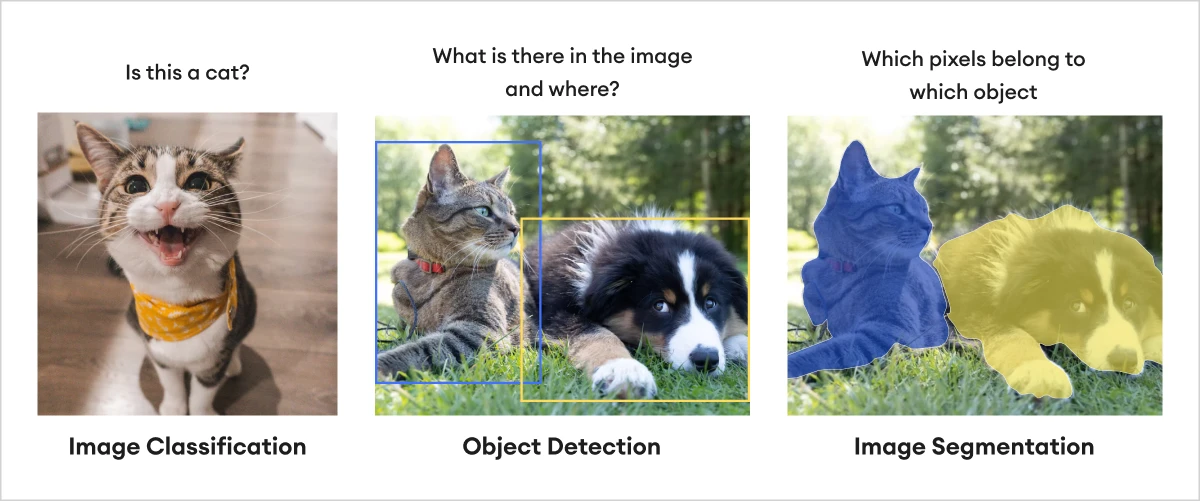
\includegraphics[width=1.07\textwidth,height=0.6\textheight,keepaspectratio]{images/segmentation/segment-intro.png}
    \end{figure}
\end{frame}

\begin{frame}{Computer Vision Tasks}
    \begin{figure}
        \centering
        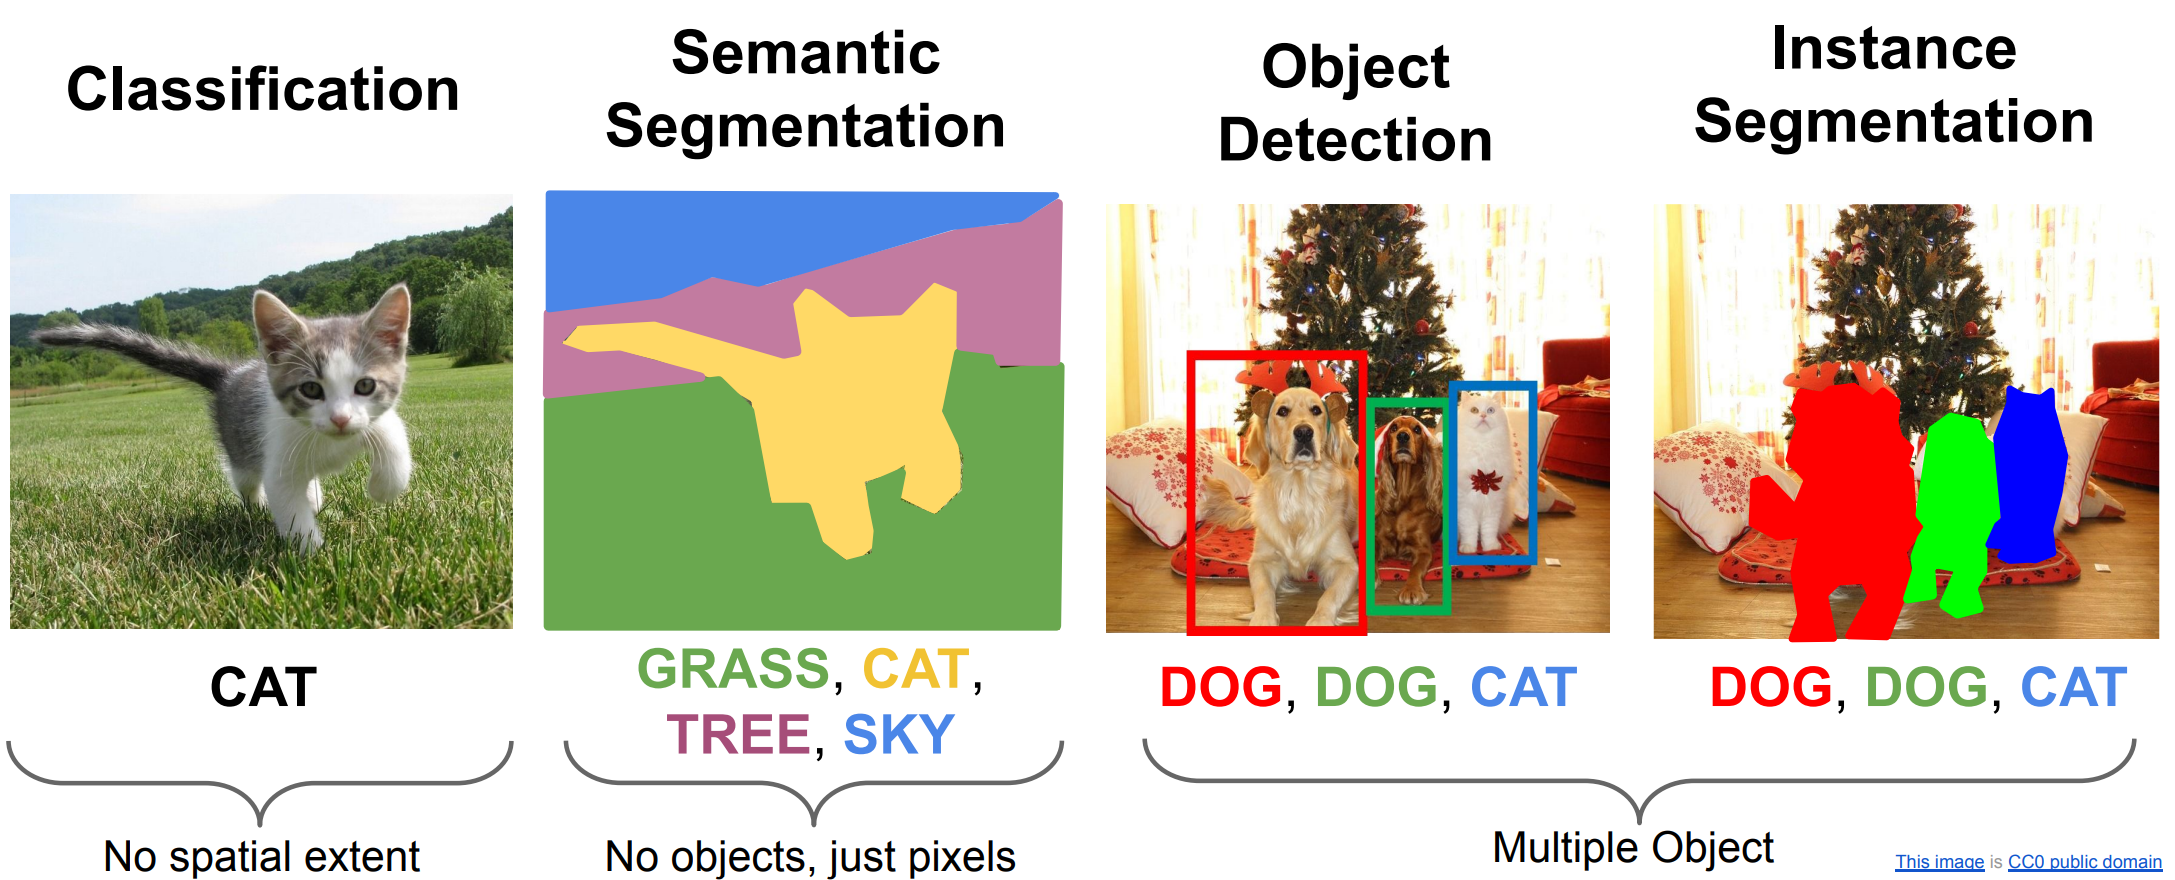
\includegraphics[width=1.0\textwidth,height=0.6\textheight,keepaspectratio]{images/segmentation/tasks.png}
    \end{figure}
    \begin{itemize}
        \item \textbf{Classification:} Identify the main object in an image.
        \item \textbf{Detection:} Locate objects with bounding boxes.
        \item \textbf{Segmentation:} Classify each pixel to delineate object boundaries.
    \end{itemize}
\end{frame}

\begin{frame}{Challenges in Segmentation}
    \begin{itemize}
        \item \textbf{Pixel-level labeling is labor-intensive}
        \item Varying object size and shape
        \item Occlusion and overlapping objects
        \item Class imbalance (background vs. object)
    \end{itemize}
\end{frame}